%Cyclone II EP2C35F672C6
\documentclass[a4paper]{report}
	%	Pacotes a serem usados
	\usepackage[latin1]{inputenc}
	\usepackage[brazil]{babel}
	\usepackage{a4wide}
	\usepackage{graphicx}
	\usepackage[pdftex]{hyperref}
	\hypersetup{
		pdftex,
	  pdftitle = {Relat�rio Sistemas Digitais - Consumo instant�neo de combust�vel},
	  pdfkeywords = {sistemas digitais, ufsc, combust�vel, consumo},
	  pdfauthor = {Bruno Luiz da Silva \\ Gustavo Fernandes},
	  colorlinks=true,
	 	citecolor=black,
	 	filecolor=black,
	 	urlcolor=black,
	 	linkcolor=black
	}
		
	%	In�cio do relat�rio (corpo do documento)
	\begin{document}
		%	Informa��es do relat�rio
		\title{Relat�rio do projeto de sistemas digitais \\ Consumo instant�neo de combust�vel}
		\author{Bruno Luiz da Silva \\ Gustavo Fernandes}
		
		%	Cria capa do relat�rio
		\begin{titlepage}
			\maketitle
		\end{titlepage}
		
		\tableofcontents
		
		\chapter{Introdu��o}
			O projeto de consumo instant�neo de combust�vel, realizado na disciplina de sistemas digitais (EEL 7020) no segundo semestre de 2011, consiste em adquirir a dist�ncia percorrida e a inje��o de combust�vel e multiplicar ambos para obter o consumo de combust�vel. Para tal foi utilizado um FPGA - Field-programmable gate array e a linguagem VHDL para construir o dispositivo que realiza tal opera��o. O projeto tem como objetivo aprimorar o conhecimento da equipe no �rea de FPGAs e VHDL assim como dar uma oportunidade para aplicar conceitos te�ricos na pr�tica.
		\chapter{Desenvolvimento e testes do medidor de consumo de combust�vel}
			%checar tabela de estados soma_mantissa


\section{Realiza��o de multiplica��es com n�mero em ponto flutuante}
Os dados que ser�o dados para o circuito ser�o todos em ponto flutuante, sendo necess�rio deixar claro como funcionam as multiplica��es com tais n�meros. Os n�meros em ponto flutuante permitem a representa��o de n�meros reais de forma digital. Para representar um decimal em bin�rio temos algo parecido parecido com a nota��o cient�fica, sendo que para tal o n�mero ser� dividido em expoente e mantissa. Exemplo disso � o n�mero 52.125. Ficaria $0.52125 * 10^{2}$ em nota��o cient�fica. Em bin�rio acontece algo semelhante. O n�mero fica representado como 110100.001 e ap�s isso � necess�rio normalizar o n�mero que deixar�-o no formato $0.MMMM * 2^E$, sendo MMMM a mantissa e E o expoente. O expoente � o n�mero de deslocamentos que foram necess�rios para deix�-lo nesse formato. No exemplo do 52.125 ele ficaria $0.110100001 * 2^6$. Seguem mais exemplos. \\
\begin{itemize}
	\item[-]$3.5  \rightarrow 0011.1000 \rightarrow 0.11100000 \cdot  2^{0010}$
	
	\item[-]$20.125  \rightarrow 10100.001 \rightarrow 0.10100001 \cdot 2^{0101}$
	
	\item[-]$15.0625 \rightarrow 1111.0001 \rightarrow 0.11110001 \cdot 2^{0100}$
	
	\item[-]$17.0 \rightarrow 10001.0 \rightarrow 0.10001 \cdot  2^{0101}$
	
	\item[-]$7.5 \rightarrow 111.1 \rightarrow 0.1111 \cdot 2^{0011}$
	
	\item[-]$5.125 \rightarrow 101.001 \rightarrow 0.101001 \cdot  2^{0011}$
	
	\item[-]$2.75 \rightarrow 10.11 \rightarrow 0.1011 \cdot  2^{0010}$
	
	\item[-]$5.225 \rightarrow 10.001110011001... \rightarrow 0.10001110011001... \cdot  2^{0010}$
	
	\item[-]$0.80 \rightarrow 0.11001100110011... \rightarrow 0.11001100110011... \cdot  2^{0000}$

\end{itemize}
\\
Para realizar a multiplica��o de n�meros de ponto flutuante s�o necess�rios dois passos.\\
\begin{enumerate}
	%begin{description}
	\item[\bf{1}]{Soma-se os expoentes e obt�m-se o expoente}
	\item[\bf{2}]{Realiza-se a multiplica��o bin�ria das mantissas e obt�m-se as mantissas}
\end{enumerate} \\

O primeiro passo � realizado como em multiplica��es decimais. Quando se tem dois n�meros multiplicados ambos pela mesma base, pode se somar os expoentes das bases. Como no exemplo:
	\begin{center}
		$(1 \cdot 10^2) \cdot (1 \cdot 10^3) = 1 \cdot 10^{(2+3)}&$
	\end{center}

No segundo passo � realizada a multiplica��o bin�ria das mantissas. Um exemplo de uma multiplica��o bin�ria 0010 (2) e 0011 (3). A multiplica��o bin�ria � muito semelhante a decimal. Segue o exemplo:
	
	\\
	\begin{figure}[!h]
		\centering
		\includegraphics[scale=.3]{multiplicacao.pdf}
	\end{figure}
	\\
	
Ap�s efetuada a multiplica��o das mantissas voc� ter� ent�o os expoentes e mantissa, tendo assim o n�mero em ponto flutuante. Nesse projeto � preciso normalizar esse n�mero e para isso � necess�rio deixar o MSB igual a um. Para tal deslocam-se todos os n�meros da mantissa para a esquerda at� atingir tal ponto. Assim, pega-se o n�mero de deslocamentos e decrementa-se do expoente, tendo assim o n�mero em ponto flutuante normalizado.

\section{Revis�o te�rica de sistemas digitais}

Alguns conceitos das aulas te�ricas de sistemas digitais valem ser revistos. O mais b�sico diz em rela��o ao que � um bin�rio e o que � o MSB e o LSB do bin�rio. Resumindo, um n�mero bin�rio � representado por 0s e 1s e cada um desses � m�ltiplicado por $2^{(n-1)}$. N � o n�mero de bits (0s ou 1s) que o bin�rio possui. Exemplo disso � o bin�rio que representa 137. Ele � representado por ``10001001'', isso �, 8 bits, logo para converter de volta para decimal tem-se 1\cdot2^7 + 0\cdot2^6 + 0\cdot2^5 + 0\cdot2^4 + 1\cdot2^3 + 0\cdot2^2 + 0\cdot2^1 + $1\cdot2^0$ que resulta em 137. 

O LSB, \textit{Least Significant Bit}, � o bit mais a direita do n�mero bin�rio e o MSB, \textit{Most Significant Bit}, � o bit mais a esquerda do n�mero bin�rio. O MSB � o mais significante por ele ser o bit de maior valor. Pegue por exemplo o valor bin�rio de 137. O MSB ser� o '1' da esquerda e ele vale $2^7$ e o LSB ser� o '1' mais a direita, que vale 2^0.

Outro conceito importante � o de registradores. Eles nada mais s�o que um conjunto de flip-flops, sendo que esses s�o componentes que s�o utilizados para armazenar dados quando o clock est� na borda de subida. Esse banco de flip-flops chamado registrador em alguns casos possui outros recursos como deslocamento de bits, podendo desloca-los tanto para direita quanto para esquerda.

Ainda h� o comparador, contador e somador, todos utilizados nesse projeto. O comparador � utilizado para comparar dois dados bin�rios. Pode ser utilizado com um contador criando assim um la�o. Enquanto a sa�da do contador n�o for a desejada o comparador n�o acusar� nada, por�m quando for ent�o ele dar� um sinal para tal. O contador a cada opera��o incrementa, normalmente, um bit a seu registrador interno e este � colocado na sa�da. Internamente ele possui um somador.

Os somadores possuem normalmente v�rios blocos para adi��o (sendo que o n�mero desses blocos � proporcional ao n�mero de bits da sa�da) os quais se chamam \textit{full-adders} e cada um considera o \textit{carry} anterior. Por exemplo, se voc� soma '1' + '1' tem-se ``10''. S� que se voc� fizer a conta a m�o voc� ter� que '1'+'1' ser� '0' e que o \textit{carry} gerado ser� '1'. O somador usa esse \textit{carry} para as somas subsequentes at� ter a soma total. Para checar se houve ou n�o overflow cria-se um XOR entre o �ltimo e pen�ltimo \textit{carry}.

J� a m�quina de estados (\textit{Finite State Machine - FSM}) � utilizada para controlar os componentes dos projetos. A cada estado ela envia um valor l�gico para alguma porta de algum componente, habilitando ou executando alguma opera��o nesse, quando algum pr�-requisito for executado (exemplo: na subida de clock $\to$  mudar de estado). Um exemplo � uma m�quina de estados de uma m�quina de refrigerantes, que s� sair� do estado inicial quando for inserida uma moeda. Assim que for inserida ela mudar� de estado e enviar� um comando para um registrador avisando o valor que foi colocado na m�quina.

Por fim h� o decodificador, que possui um funcionamento simples. Quando enviado um n�mero bin�rio, ele a interpretar� e ent�o ter� somente uma de suas sa�das ativadas. O n�mero de sa�das � $2^n$, sendo n o n�mero de bits do n�mero enviado e a sa�da a ser ativada ser� o n�mero bin�rio enviado + 1. Por exemplo, se a entrada for 101 (cinco em decimal) ent�o somente a sexta sa�da (5 + 1) ter� valor l�gico alto.

\section{Fluxo do projeto}

O projeto foi realizado em etapas. A primeira foi pensar no funcionamento das multiplica��es de n�meros de ponto flutuante. Assim que descoberto como � tal processo a equipe hipotetizou como seria o circuito. Para tal foram checadas tamb�m as refer�ncias deixadas pelo professor em seu \textit{website} e utilizou-se o conhecimento dado nas aulas te�ricas. A primeira modifica��o da refer�ncia deixada pelo professor foi a troca de dois registradores de 8 bits por um de 16 bits, que seria mais facilmente desenvolvido em VHDL. Al�m disso, a passagem do multiplicador pelo registrador de 8 bits restante se fez desnecess�rio visto que seria mais f�cil construir um bloco de decodifica��o e ele faria as etapas que passariam pelo registrador de 8 bits.

Ap�s desenvolvida as id�ias de como seria o circuito, iniciou-se o desenvolvimento do circuito em VHDL. Essa linguagem, \textit{VHSIC hardware description language}, � utilizada para descrever um hardware e assim ``constru�-lo''. Esse c�digo, no atual projeto, ser� utilizado para descrever qual ser� o harware que ser� implementado na kit de desenvolvimento Altera DE 2 que utiliza a FPGA Cyclone II EP2C35F672C6. A ferramenta utilizada para desenvolver o projeto foi o Altera Quartus II 9.1 SP2, onde criou-se os VHDLs respons�veis por cada componente, al�m de toda a simula��o. Vale constar que o uso da vers�o 9.1, que n�o � a mais atual, � devido a ferramenta de simula��o n�o estar mais presente nas vers�es atuais.

Cada componente foi desenvolvido, comentado e simulado separadamente, possibilitando assim a avalia��o de cada um e evitando problemas ao procurar erros no projeto principal. Ap�s finalizados, utilizou-se o recurso ``port map'' do VHDL para conectar todos os componentes num componente principal, constituindo assim o calculador de consumo. Foram realizadas v�rias simula��es e assim que atestado o funcionamento do projeto, continuou-se a comentar o c�digo e procurar poss�veis erros.

Por fim, inicializou-se a cria��o desse relat�rio afim de explicar como ocorreu o projeto. Para cri�-lo foi utilizado o padr�o \LaTeX, pretendo aprender mais sobre tal padr�o. \\

\section{Implementa��o do circuito}
Para criar tal circuito foram utilizados registradores, deslocadores, contadores, somadores, comparadores, decodificadores e por fim uma m�quina de estados. Os registradores utilizados foram um de oito bits, muito simples, s� utilizado para armazenar valor e outro de dezesseis bits mais um, pois houve a necessidade de armazenar o carry do somador anterior logo foi adicionado um bit a mais. Esse registrador � muito mais complexo que o primeiro, pois possui dois deslocadores e um contador.

Um dos deslocadores desse registrador serve para deslocar os bits a direita, utilizado na multiplica��o (soma e deslocamento). J� o segundo deslocador � para deslocar os bits a esquerda, permitindo assim a normaliza��o da mantissa. Vale notar que a cada deslocamento desse � adicionado um num contador que ao final dar� o n�mero de deslocamentos que foram necess�rios para normalizar o n�mero, o que influenciar� no resultado do expoente.

Al�m disso h� um somador anexado a um comparador, que checar� se o LSB � '0' ou '1' e a partir disso far� a soma de multiplicando com parte alta do registrador de 16 bits ou n�o executar� nada. Isso � crucial para realizar a multiplica��o, afinal o processo todo se d� por soma e deslocamento, sendo que a soma � feita aqui e o deslocamento, como dito anteriormente, no registrador.

Ainda h� a parte do expoente. Nele existir� um somador que far� a adi��o entre os dois expoentes dados e armazenar� esses dados at� que a mantissa seja normalizada para que o n�mero de deslocamentos possa ser decrementado da soma anterior e assim ter o expoente final.

Segue um lista com mais detalhes sobre cada componente.

\begin{description}
	\item[Consumo combust�vel: ]esse ser� o bloco ``top-entity'' onde ser�o conectadas as chaves (SW), bot�es (KEY), clock (CLOCK\_50) e LEDs (LEDG e LEDR). Tamb�m deve-se notar que ser� aqui que todos os outros componentes ser�o conectados e assim receber�o os dados do usu�rio. O usu�rio colocar� um valor de oito bits inicialmente (multiplicando) e apertar� o bot�o KEY(1) que amazenar� tal valor no registrador de 8 bits. Ap�s o usu�rio soltar o bot�o ent�o o componente aguardar� a inser��o do outro valor (multiplicador) e consequente pressionamento de KEY(1). Ap�s feito	isso ent�o o componente aguardar� os valores dos expoentes, sendo de 4 bits cada e ambos ser�o inseridos nas mesmas chaves (SW). Para tal SW(7 downto 4) ser� um expoente e SW(3 downto 0) ser� outro. Assim que for apertado KEY(1) ent�o as opera��es de multiplica��o ser�o realizadas. Somar�-se os dois expoentes, realizar�-se o processo de multiplica��o da mantissa e posterior normaliza��o e por fim haver� a subtra��o do n�mero de deslocamentos que foram necess�rios na normaliza��o com o atual valor da soma dos dois expoentes. Tem-se assim o valor final, que ter� a mantissa representada em LEDG(7 downto 0) e expoentes em LEDR. Caso houver overflow ele ser� indicado em LEDG(8). 
	
	Os sinais utilizados ser�o apenas para conectar um componente � outro, com excess�o de mantissa\_out(15 downto 8) que ser� ligado a sa�da LEDG(7 downto 0), exponent\_out(3 downto 0) que ser� ligado a sa�da LEDR e exponent\_out(4) que ser� ligado a sa�da LEDG(8). Este �ltimo indicar� se houve ou n�o overflow, utilizando a id�ia de que o expoente s� pode ir de 0 t� 15, isso �, de ``0000'' at� ``1111''. Se esse valor for ultrapassado ent�o ter�-se no m�nimo '1' no MSB de exponent\_out, algo como ``10000'' (representa��o bin�ria de 16).
	
	\item[Multiplicador: ]bloco onde ser� realizada a multiplica��o das duas mantissas. Para tal, o usu�rio entrar� com os dados de 8 bits e para controlar para quais componentes esses dados ir�o, ser� utilizado o input\_control (logo abaixo haver� uma descri��o detalhada dele), sendo que os ``arguments'' ser�o enviados por uma FSM e habilitar� os componentes corretos no momento certo. Deve-se primeiramente carregar o registrador de 8 bits com esses dados (reg\_8 / ``001''), depois carregar a parte baixa do registrador de 16 bits (reg16 /  ``010'') e ent�o iniciar a adi��o e/ou deslocamento.
	
Para tal o componente de soma dever� ser ativado, sendo que o mesmo argumento ativa o armazenamento de dados para a parte alta registrador de 16 bits (``011''). Essa opera��o envia a sa�da da parte alta do registrador de 16 bits para a entrada ``b'' do somador e na entrada ``a'' tem-se o valor do registrador de 8 bits. Ainda � enviado o �ltimo bit presente no reg\_16 pois	caso ele for 0 os valores armazenados ser�o apenas deslocados a direita e caso for 1 ent�o soma-se as duas entradas e desloca-se os valores armazenados. Para realizar o deslocamento usa-se o argumento ``100''.

O processo de adi��o e deslocamento deve ser efetuado oito vezes. Quando esse processo terminar tem-se o produto das mantissas, por�m para o projeto ser� necess�rio normalizar a mantissa. Para tal o primeiro bit do produto (MSB) deve ser 1 e para isso � preciso avaliar esse bit e caso for 0 desloca-se o valor armazenado para a esquerda. Essa opera��o � realizada pelo registrador de 16 bits (argumento: ``101''). Cada vez que houver o deslocamento ser� incrementado 1 em um contador interno. Ap�s o MSB for 1 ent�o finaliza-se o processo e ter�-se o valor de vezes que o n�mero foi deslocado. Esse resultado ser� utilizado para decrementar o expoente posteriormente.

Os sinais utilizados em sua maioria ser�o somente para conectar as entradas e sa�das dos componentes entre si, com excess�o do reg16out onde ser� ligado na sa�da q do Multiplicador e exp que ser� ligado na sa�da exp\_nor.

\item[Input\_control: ]esse componente n�o � de controle, afinal ele faz um papel de decodificador, mas para facilitar o entendimento foi colocado essa nomenclatura. A partir de um argumento ele habilitar� somente os componentes corretos, sendo que esses ser�o enviados por uma m�quina de estados, a qual realmente controla o circuito. Na entrada ``a'' estar�o conectadas as chaves SW e em ``reg'' estar� conectada a parte alta do registrador de 16 bits. Suas sa�das ser�o conectadas diretamente nas entradas que habilitam as opera��es dos componentes (armazenamento, deslocamento e outras). Segue uma tabela com a especifica��o de o que cada uma faz.

\\
\begin{center}
\begin{tabular}{|l|p{3cm}|l|l|l|l|l|l|}
\hline
\multicolumn{1}{|c|}{\bf{Argumento}} & \multicolumn{1}{p{3cm}|}{\bf{Descri��o}} & \multicolumn{1}{c|}{\bf{l1}} & \multicolumn{1}{c|}{\bf{l2}} & \multicolumn{1}{c|}{\bf{s1}} & \multicolumn{1}{c|}{\bf{shift}} & \multicolumn{1}{c|}{\bf{n1}} & \multicolumn{1}{c|}{\bf{q}} \\ 
\hline
\multicolumn{1}{|c|}{000} & \multicolumn{1}{p{3cm}|}{nada} & \multicolumn{1}{c|}{0} & \multicolumn{1}{c|}{0} & \multicolumn{1}{c|}{0} & \multicolumn{1}{c|}{0} & \multicolumn{1}{c|}{0} & \multicolumn{1}{c|}{} \\ 
\hline
\multicolumn{1}{|c|}{001} & \multicolumn{1}{p{3cm}|}{carrega reg. de 8 bits} & \multicolumn{1}{c|}{1} & \multicolumn{1}{c|}{0} & \multicolumn{1}{c|}{0} & \multicolumn{1}{c|}{0} & \multicolumn{1}{c|}{0} & \multicolumn{1}{c|}{} \\ 
\hline
\multicolumn{1}{|c|}{010} & \multicolumn{1}{p{3cm}|}{carrega parte baixa do reg. de 16 bits} & \multicolumn{1}{c|}{0} & \multicolumn{1}{c|}{0} & \multicolumn{1}{c|}{1} & \multicolumn{1}{c|}{0} & \multicolumn{1}{c|}{0} & \multicolumn{1}{c|}{} \\ 
\hline
\multicolumn{1}{|c|}{011} & \multicolumn{1}{p{3cm}|}{ativa somador e parte alta do registrador de 16 bits} & \multicolumn{1}{c|}{0} & \multicolumn{1}{c|}{1} & \multicolumn{1}{c|}{0} & \multicolumn{1}{c|}{0} & \multicolumn{1}{c|}{0} & \multicolumn{1}{c|}{``reg''} \\ 
\hline
\multicolumn{1}{|c|}{100} & \multicolumn{1}{p{3cm}|}{habilitar� deslocamento para esquerda do registrador de 16 bits} & \multicolumn{1}{c|}{0} & \multicolumn{1}{c|}{0} & \multicolumn{1}{c|}{0} & \multicolumn{1}{c|}{1} & \multicolumn{1}{c|}{0} & \multicolumn{1}{c|}{} \\ 
\hline
\multicolumn{1}{|c|}{101} & \multicolumn{1}{p{3cm}|}{normaliza os dados do reg. de 16 bits} & \multicolumn{1}{c|}{0} & \multicolumn{1}{c|}{0} & \multicolumn{1}{c|}{0} & \multicolumn{1}{c|}{0} & \multicolumn{1}{c|}{1} & \multicolumn{1}{c|}{} \\ 
\hline
\end{tabular}
\end{center} \\

\item[Registrador de 8 bits: ]guardar� o valor de 8 bits que for dado para a entrada ``d'', nesse caso o multiplicando, quando for dado um valor l�gico alto para a entrada ``enable''. A sa�da (``q'') ser� o valor armazenado quando o enable foi dado como alto.

\item[Somador: ]este realizar� a soma entre o valor do registrador de 8 bits (entrada a) com a parte alta do registrador de 16 bits (entrada b) quando seu ``enable'' estiver com valor l�gico alto e o MSB do registrador de 16 bits for '1', o qual ser� dado na entrada ``control''. Caso contr�rio, quando ``enable'' for alto ent�o o componente s� copiar� o valor da parte alta para o registrador direto para sua sa�da, n�o executando nenhuma opera��o. A sa�da ser� o resultado gerado por uma dessas duas condi��es.

\item[Registrador de 16 bits (+ 1): ]ao final ser� ele que guardar� o produto das mantissas. Inicialmente ser�o dados os valores do multiplicador na entrada ``chaves'' e estes ser�o guardados na parte baixa do registrador (7 downto 0). Para tal ser� necess�rio dar um valor l�gico alto para ``start''. Para carregar o valor que vier do somador ter�-se que conectar a sa�da do contador na entrada ``soma'' e colocar um valor l�gico alto em ``load'' para assim o valor ser� guardado na parte alta do registrador (15 downto 8). 

Como esse bloco ser� usado para um multiplicador ent�o ser� necess�rio que o valor seja deslocado ap�s a opera��o do componente ``somador''. Para realizar isto ser� necess�rio dar um valor l�gico alto para ``shift'' a cada deslocamento desejado.

	A normaliza��o far�-se necess�ria neste projeto, logo ``normalize'' deve receber um valor l�gico alto para que se inicie a normaliza��o. Nesse processo o signal ``works'' tornar�-se 1 e enquanto o MSB n�o for 1, ``works'' permanecer� em 1, desabilitando qualquer outra opera��o do componente. Quando a opera��o estiver conclu�da ter�-se o n�mero normalizado e ``exp'' armazenar� o n�mero de deslocamentos que foram necess�rios.
	
	Vale notar que o \emph{+1} no t�tulo do componente deve-se ao bit extra colocado no registrador para n�o acontecerem problemas com o carry da soma entre multiplicando e parte alta do registrador.
	
	Os sinais utilizados, como \emph{aux}, \emph{exp\_aux} e \emph{works}, servir�o, repectivamente, para armazenar os resultados, armazenar quantas vezes foi deslocado o produto e para ativar a normaliza��o.
	
	\item[Expoente: ]esse ser� o componente respon�vel para dar o expoente da multiplica��o, que se faz necess�rio por ser uma multiplica��o de n�meros de ponto flutuante. Para tal o usu�rio entrar� com os expoentes nas entradas ``a'' e ``b'' al�m de dar o valor ``110'' para o ``argument'' para assim realizar a soma de ambos. Para previnir casos onde houver uma soma que extrapole o valor ``1111'' (15 em decimal) ent�o foi adicionado um bit extra na sa�da para armazenar o poss�vel valor extra. Em algum momento o ``argument'' ser� ``111'' e ent�o ser� realizada a subtra��o entre o valor da soma dos expoentes com o n�mero de deslocamentos realizados para normalizar a mantissa, que ser� dado na entrada ``normal''. Ap�s isso ent�o tem-se o expoente final, por�m ele deve estar na faixa de ``0000'' a ``1111'' (0 a 15 em decimal), pois caso extrapole essa faixa ele n�o poder� apresentar o valor correto nos LEDs designados sendo assim um caso de \textit{overflow}, que ativar� o LED(8) por meio do bit extra que existe no componente (q(4)).
	
	O sinal utilizado (aux) ser� apenas para armazenar os dados e em alguns momentos modific�-los.
	
\end{description}

Essa foi uma descri��o de quase todos os componentes. Ainda h� a maquina de estados, que ser� tratada na pr�xima se��o. Segue abaixo um diagrama do circuito.

\\
\begin{figure}
	\includegraphics[width=17cm]{blocos.pdf}
\end{figure}
\\

\newpage

\section{M�quina de estados (Finite State Machine)}
	Para o projeto foi criada uma m�quina de estados para controlar os componentes e registradores. No caso os sinais de sa�da de FSM ser�o ``argumentos'' que dentro dos blocos de multiplica��o e expoente ser�o interpretados e habilitar�o alguns componentes ou dar�o algum comando para o componente funcionar como desejado (exemplo: deslocar bits para direita ou para esquerda).
	
	No diagrama � poss�vel checar quais s�o os sinais de sa�da dele (arg) e pode-se verificar o que cada um faz na tabela %inserir tabela%. 
	A tabela que segue representa a transi��o dos estados e v�-se exatamente o comportamento da FSM a partir de certos par�metros como do \emph{enter}, \emph{reset}, \emph{count} e \emph{reg\_control}. \\ 
\begin{center}	\footnotesize \begin{tabular}{|l|l|l|l|l|l|}
\hline
\multicolumn{1}{|c|}{\bf{Estado atual}} & \multicolumn{1}{c|}{\bf{Pr�ximo estado}} & \multicolumn{1}{c|}{\bf{K(1)}} & \multicolumn{1}{c|}{\bf{K(0)}} & \multicolumn{1}{c|}{\bf{COUNT}} & \multicolumn{1}{c|}{\bf{REG\_CONTROL}} \\ 
\hline
\multicolumn{1}{|c|}{Inicial} & \multicolumn{1}{c|}{Carrega\_reg8} & \multicolumn{1}{c|}{1} & \multicolumn{1}{c|}{0} & \multicolumn{1}{c|}{X} & \multicolumn{1}{c|}{X} \\ 
\hline
\multicolumn{1}{|c|}{Carrega\_reg8} & \multicolumn{1}{c|}{Dummy1} & \multicolumn{1}{c|}{0} & \multicolumn{1}{c|}{1} & \multicolumn{1}{c|}{X} & \multicolumn{1}{c|}{X} \\ 
\hline
\multicolumn{1}{|c|}{Carrega\_reg8} & \multicolumn{1}{c|}{Carrega\_reg8} & \multicolumn{1}{c|}{1} & \multicolumn{1}{c|}{1} & \multicolumn{1}{c|}{X} & \multicolumn{1}{c|}{X} \\ 
\hline
\multicolumn{1}{|c|}{Dummy1} & \multicolumn{1}{c|}{Carrega\_reg16} & \multicolumn{1}{c|}{1} & \multicolumn{1}{c|}{1} & \multicolumn{1}{c|}{X} & \multicolumn{1}{c|}{X} \\ 
\hline
\multicolumn{1}{|c|}{Dummy1} & \multicolumn{1}{c|}{Dummy1} & \multicolumn{1}{c|}{0} & \multicolumn{1}{c|}{1} & \multicolumn{1}{c|}{X} & \multicolumn{1}{c|}{X} \\ 
\hline
\multicolumn{1}{|c|}{Carrega\_reg16} & \multicolumn{1}{c|}{Dummy2} & \multicolumn{1}{c|}{0} & \multicolumn{1}{c|}{1} & \multicolumn{1}{c|}{X} & \multicolumn{1}{c|}{X} \\ 
\hline
\multicolumn{1}{|c|}{Carrega\_reg16} & \multicolumn{1}{c|}{Carrega\_reg16} & \multicolumn{1}{c|}{1} & \multicolumn{1}{c|}{1} & \multicolumn{1}{c|}{X} & \multicolumn{1}{c|}{X} \\ 
\hline
\multicolumn{1}{|c|}{Dummy2} & \multicolumn{1}{c|}{Soma\_expoentes} & \multicolumn{1}{c|}{1} & \multicolumn{1}{c|}{1} & \multicolumn{1}{c|}{X} & \multicolumn{1}{c|}{X} \\ 
\hline
\multicolumn{1}{|c|}{Dummy2} & \multicolumn{1}{c|}{Dummy2} & \multicolumn{1}{c|}{0} & \multicolumn{1}{c|}{1} & \multicolumn{1}{c|}{X} & \multicolumn{1}{c|}{X} \\ 
\hline
\multicolumn{1}{|c|}{Soma\_expoentes} & \multicolumn{1}{c|}{Soma\_mantissa} & \multicolumn{1}{c|}{0} & \multicolumn{1}{c|}{1} & \multicolumn{1}{c|}{X} & \multicolumn{1}{c|}{X} \\ 
\hline
\multicolumn{1}{|c|}{Soma\_expoentes} & \multicolumn{1}{c|}{Soma\_expoentes} & \multicolumn{1}{c|}{1} & \multicolumn{1}{c|}{1} & \multicolumn{1}{c|}{X} & \multicolumn{1}{c|}{X} \\ 
\hline
\multicolumn{1}{|c|}{Soma\_mantissa} & \multicolumn{1}{c|}{Desloca\_mantissa} & \multicolumn{1}{c|}{X} & \multicolumn{1}{c|}{1} & \multicolumn{1}{c|}{count != 0000} & \multicolumn{1}{c|}{X} \\ 
\hline
\multicolumn{1}{|c|}{Soma\_mantissa} & \multicolumn{1}{c|}{Normaliza} & \multicolumn{1}{c|}{X} & \multicolumn{1}{c|}{1} & \multicolumn{1}{c|}{count = 0000} & \multicolumn{1}{c|}{X} \\ 
\hline
\multicolumn{1}{|c|}{Desloca\_mantissa} & \multicolumn{1}{c|}{Soma\_mantissa} & \multicolumn{1}{c|}{X} & \multicolumn{1}{c|}{1} & \multicolumn{1}{c|}{X} & \multicolumn{1}{c|}{X} \\ 
\hline
\multicolumn{1}{|c|}{Normaliza} & \multicolumn{1}{c|}{Expoente} & \multicolumn{1}{c|}{X} & \multicolumn{1}{c|}{1} & \multicolumn{1}{c|}{X} & \multicolumn{1}{c|}{1} \\ 
\hline
\multicolumn{1}{|c|}{Normaliza} & \multicolumn{1}{c|}{Normaliza} & \multicolumn{1}{c|}{X} & \multicolumn{1}{c|}{1} & \multicolumn{1}{c|}{X} & \multicolumn{1}{c|}{0} \\ 
\hline
\multicolumn{1}{|c|}{Expoente} & \multicolumn{1}{c|}{Final} & \multicolumn{1}{c|}{X} & \multicolumn{1}{c|}{1} & \multicolumn{1}{c|}{X} & \multicolumn{1}{c|}{X} \\ 
\hline
\multicolumn{1}{|c|}{Final} & \multicolumn{1}{c|}{Final} & \multicolumn{1}{c|}{X} & \multicolumn{1}{c|}{1} & \multicolumn{1}{c|}{X} & \multicolumn{1}{c|}{X} \\ 
\hline
\multicolumn{1}{|c|}{Final} & \multicolumn{1}{c|}{Inicial} & \multicolumn{1}{c|}{X} & \multicolumn{1}{c|}{0} & \multicolumn{1}{c|}{X} & \multicolumn{1}{c|}{X} \\ 
\hline
\end{tabular} \\ \end{center}
\emph{Observa��o: ENTER e K(1) referem-se a KEY(1) e RESET e K(0) a KEY(0)}\\

\linebreak

 Segue uma descri��o detalhada do que ocorre em cada estado:
\begin{description}
	\item[Inicial: ]esse ser� o estado inicial, onde n�o haver� nenhuma sa�da. S� vira para esse estado se o \emph{RESET} for pressionado.
	
	\item[Carrega\_reg8: ]respons�vel por carregar o registrador de 8 bits quando \emph{ENTER} for pressionado pela primeira vez, guardando o valor do multiplicando, que dever� estar configurado nas chaves. Para tal sua sa�da ser� ``001''.
	
	\item[Dummy1: ]ser� encarregado de aguardar que \emph{ENTER} seja despressionada, pois caso n�o existisse esse estado ent�o em apenas alguns segundos todos os registradores estariam carregados com o mesmo dado.
	
	\item[Carrega\_reg16: ]respons�vel por carregar o registrador de 16 bits quando \emph{ENTER} for pressionado pela segunda vez, guardando o valor do multiplicador na parte baixa do registrador (7 downto 0). Para isso sua sa�da ser� ``010''.
	
	\item[Dummy2: ]ser� encarregado de aguardar que \emph{ENTER} seja despressionada, novamente.
	
	\item[Soma\_expoentes: ]quando \emph{ENTER} for pressionada pela terceira vez ent�o os valores que estiverem nas chaves ser�o enviados para um somador que somar� os primeiros 4 bits com os 4 �ltimos (7 downto 4 e 3 downto 0) para que se tenha o expoente. Para tal a sa�da da FSM ser� ``101'' e al�m dos processo descritos acima ela inicializar� um contador (\emph{count}) em oito (``1000'').
	
	\item[Soma\_mantissa: ]na multiplica��o devem ser executadas somas e deslocamentos. Esse estado ser� respons�vel por fazer a poss�vel soma entre valores da parte alta do registrador de 16 bits (15 downto 8) e registrador de 8 bits (multiplicando), por�m somente enquanto o contador, antes inicializado, for diferente de zero (``0000''). Quando o contador for zero ent�o o pr�ximo estado n�o ser� mais ``Desloca\_mantissa'', mas sim ``Normaliza''. Para realizar a soma a sa�da dever� ser ``011''.
	
	\item[Desloca\_mantissa: ]essa parte ser� respons�vel por deslocar os dados do registrador de 16 bits, fazendo parte de mais um passo da opera��o de multiplica��o. Ainda nesse estado o contador � decrementado em um, pois s� assim em algum momento o contador \emph{count} ser� zero. A sa�da desse estado ser� ``100''.
	
	\item[Normaliza: ]ap�s a multiplica��o ter sido efetuada e os expoentes somados temos o n�mero em ponto flutuante, por�m � necess�rio ainda normalizar o n�mero, isso �, o MSB dever� ser igual � '1'. Para tal a sa�da ser� ``101'' que far� com que o registrador de 16 bits inicialize a normaliza��o. A sa�da desse estado para ``Expoente'' s� ocorrer� quando reg\_control for igual � '1' (ele � o MSB citado).
	
	\item[Expoente: ]depois da normaliza��o � necess�rio subtrair o n�mero de deslocamentos com a soma dos expoentes efetuadas anteriormente. Para tal a sa�da da FSM ser� ``111''.
	
	\item[Final: ]chegou ao final das opera��es e o resultado final � disponibilizado. S� sair� desse estado caso for pressionado o \emph{RESET}.
	
\end{description}

A tabela a seguir resume quais ser�o as sa�das da m�quina de estados, facilitando o encontro de poss�veis erros.
\\
\begin{center}
\begin{tabular}{|l|l|l|}
\hline
\multicolumn{1}{|c|}{\bf{Estado}} & \multicolumn{1}{c|}{\bf{Sa�da (arg)}} & \multicolumn{1}{c|}{\bf{COUNT}} \\ 
\hline
\multicolumn{1}{|c|}{Inicial} & \multicolumn{1}{c|}{000} & \multicolumn{1}{c|}{X} \\ 
\hline
\multicolumn{1}{|c|}{Carrega\_reg8} & \multicolumn{1}{c|}{001} & \multicolumn{1}{c|}{X} \\ 
\hline
\multicolumn{1}{|c|}{Dummy1} & \multicolumn{1}{c|}{000} & \multicolumn{1}{c|}{X} \\ 
\hline
\multicolumn{1}{|c|}{Carrega\_reg16} & \multicolumn{1}{c|}{010} & \multicolumn{1}{c|}{X} \\ 
\hline
\multicolumn{1}{|c|}{Dummy2} & \multicolumn{1}{c|}{000} & \multicolumn{1}{c|}{X} \\ 
\hline
\multicolumn{1}{|c|}{Soma\_expoentes} & \multicolumn{1}{c|}{101} & \multicolumn{1}{c|}{count = "1000"} \\ 
\hline
\multicolumn{1}{|c|}{Soma\_mantissa} & \multicolumn{1}{c|}{000} & \multicolumn{1}{c|}{count = "0000"} \\ 
\hline
\multicolumn{1}{|c|}{Soma\_mantissa} & \multicolumn{1}{c|}{011} & \multicolumn{1}{c|}{count != "0000"} \\ 
\hline
\multicolumn{1}{|c|}{Desloca\_mantissa} & \multicolumn{1}{c|}{100} & \multicolumn{1}{c|}{count - 1} \\ 
\hline
\multicolumn{1}{|c|}{Normaliza} & \multicolumn{1}{c|}{101} & \multicolumn{1}{c|}{X} \\ 
\hline
\multicolumn{1}{|c|}{Expoente} & \multicolumn{1}{c|}{111} & \multicolumn{1}{c|}{X} \\ 
\hline
\multicolumn{1}{|c|}{Final} & \multicolumn{1}{c|}{000} & \multicolumn{1}{c|}{X} \\ 
\hline
\end{tabular}
\end{center}

Abaixo segue um diagrama de estados que representa graficamente os estados denotados acima.

\\
		\begin{figure}[!h]
				\centering
				\includegraphics[width=10cm]{fsm.pdf}
				\caption{Diagrama da m�quina de estados}
		\end{figure}
		\\

\newpage 


\section{Resultados e simula��es}
Ap�s toda a implementa��o do circuito em VHDL foram realizadas simula��es. Para tal foi usado o pr�prio Quartus II 9.1, que ainda inclui a ferramentas para simula��es. No Quartus foi utilizada a ferramenta de simula��o, dispon�vel em \textit{Processing -> Simulator Tool}, para realizar multiplas simula��es de uma s� vez. 

Uma observa��o a ser colocada � que pela proposta do projeto permitir apenas o uso de 8 LEDs para indicar o produto haver� perda de precis�o nas multiplica��es. Al�m disso a FPGA utilizada usa sinal alto para KEY desativada e sinal baixo para KEY ativada (pressionada). Segue uma tabela de algumas simula��es realizadas.\\
\begin{center} \footnotesize \begin{tabular}{|l|l|l|l|l|l|l|l|}
\hline
\multicolumn{1}{|c|}{\bf{Multiplica��o}} & \multicolumn{1}{c|}{\bf{Mantis. 1}} & \multicolumn{1}{c|}{\bf{Exp. 1}} & \multicolumn{1}{c|}{\bf{Mantis. 2}} & \multicolumn{1}{c|}{\bf{Exp. 2}} & \multicolumn{1}{c|}{\bf{Resultado}} & \multicolumn{1}{c|}{\bf{Decimal}} & \multicolumn{1}{c|}{\bf{Esperado}} \\ 
\hline
\multicolumn{1}{|c|}{8.71 \cdot 128} & \multicolumn{1}{c|}{10001011} & \multicolumn{1}{c|}{0100} & \multicolumn{1}{c|}{10000000} & \multicolumn{1}{c|}{1000} & \multicolumn{1}{c|}{0.10001011 \cdot $2^{11}$} & \multicolumn{1}{c|}{1112} & \multicolumn{1}{c|}{1114.88} \\ 
\hline
\multicolumn{1}{|c|}{64.5 \cdot 30.6} & \multicolumn{1}{c|}{10000001} & \multicolumn{1}{c|}{0111} & \multicolumn{1}{c|}{11110100} & \multicolumn{1}{c|}{0101} & \multicolumn{1}{c|}{0.11110101 \cdot $2^{11}$} & \multicolumn{1}{c|}{1960} & \multicolumn{1}{c|}{1973.7} \\ 
\hline
\multicolumn{1}{|c|}{671.125 \cdot 64.5} & \multicolumn{1}{c|}{10100111} & \multicolumn{1}{c|}{1010} & \multicolumn{1}{c|}{10000001} & \multicolumn{1}{c|}{0111} & \multicolumn{1}{c|}{Overflow} & \multicolumn{1}{c|}{Overflow} & \multicolumn{1}{c|}{43287.56} \\ 
\hline
\multicolumn{1}{|c|}{0 \cdot 0} & \multicolumn{1}{c|}{00000000} & \multicolumn{1}{c|}{0000} & \multicolumn{1}{c|}{00000000} & \multicolumn{1}{c|}{0000} & \multicolumn{1}{c|}{00000000} & \multicolumn{1}{c|}{0} & \multicolumn{1}{c|}{0} \\ 
\hline
\multicolumn{1}{|c|}{555.125 \cdot 118.03125} & \multicolumn{1}{c|}{10001010} & \multicolumn{1}{c|}{1010} & \multicolumn{1}{c|}{11101100} & \multicolumn{1}{c|}{0111} & \multicolumn{1}{c|}{Overflow} & \multicolumn{1}{c|}{Overlow} & \multicolumn{1}{c|}{65522.098} \\ 
\hline
\multicolumn{1}{|c|}{88.8 \cdot 175.63} & \multicolumn{1}{c|}{10110001} & \multicolumn{1}{c|}{0111} & \multicolumn{1}{c|}{10101111} & \multicolumn{1}{c|}{1000} & \multicolumn{1}{c|}{11110001 \cdot $2^{14}$} & \multicolumn{1}{c|}{15424} & \multicolumn{1}{c|}{15595.94} \\ 
\hline
\end{tabular}\end{center}\\

\emph{Obs.: ``Mantis.'' significa Mantissa e ``Exp.'' significa expoente.}\\

Na tabela � poss�vel ver a perda de preciss�o que � gerada pelo circuito e como ele n�o suporta n�meros muito grandes. No caso de n�meros grandes � indicado overflow, dado no projeto pelo LEDG(8).

Os dados para simula��o s�o colocados como sinais (alto ou baixo) que forma n�meros bin�rios. Para isso � usado um arquivo chamado \textit{vector waveform} e ap�s a simula��o ter sido realizada tem-se o relat�rio. Segue o exemplo do relat�rio da multiplica��o 64.5\cdot30.6.

\\
\begin{figure}[!h]
	\centering
	\includegraphics[width=13cm]{simula1.png}
\end{figure}
\\

Quando KEY = 2, ent�o tem-se que KEY(1) � 1 e KEY(0) � 0. Isso quer dizer que KEY(0) est� sendo pressionado, fazendo com que o sistema seja reiniciado, voltando assim para o estado ``inicial''. Alguns pulsos de clocks e ent�o tem-se o armazenamento de dados no registrador de 8 bits, quando KEY = 1 (tem-se KEY(1) igual a 0 e KEY(0) igual a 1). Segue-se o estado vazio, para esperar o KEY ser despressionado ent�o tem-se o carregamento da parte baixa do registrador de 16 bits (KEY = 1 novamente). A forma de onda ficou cortada, por�m � percept�vel que ele guardou o dado pois passou do estado ``carrega\_reg16'' para ``dummy2''.

\\
\begin{figure}[!h]
	\centering
	\includegraphics[width=13cm]{simula2.png}
\end{figure}
\\

Insere-se ent�o os valores dos expoentes e pressiona-se o KEY(1), tornando KEY = 1 novamente e realizando a adi��o de ambos expoentes (checados em LEDR, pen�ltima linha da simula��o). A partir disso n�o ser� mais necess�rio pressionar nenhum bot�o. Entra-se ent�o no processo de soma e deslocamento, isso �, multiplica��o das mantissas, a qual pode ser avaliada em LEDG (anti-pen�ltima linha da simula��o).
\newpage

\\
\begin{figure}[!h]
	\centering
	\includegraphics[width=13cm]{simula3.png}
\end{figure}
\\

\\\begin{figure}[!h]
	\centering
	\includegraphics[width=13cm]{simula4.png}
\end{figure}
\\

\\\begin{figure}[!h]
	\centering
	\includegraphics[width=13cm]{simula5.png}
\end{figure}
\\

Continua-se o processo de soma e deslocamento, at� que se realize as oito vezes propostas. Ap�s a �ltima	intera��o de soma e desloca (presente na pen�ltima imagem) tem-se o processo de normaliza��o, que roda at� que MSB do registrador de 16 bits seja '1'. Ap�s isso entra-se no ``expoente'' onde realiza-se o decremento da soma dos expoentes com o n�mero de deslocamentos da normaliza��o e ent�o tem-se o resultado final, representado nos LEDG e LEDR, sendo eles mantissa e expoente respectivamente. N�o h� overflow, como pode ser visto, levando em conta que a proposta do projeto relacionava o LEDG(8) para indicar a ocorr�ncia de overflow.

O resultado, 0.11110101 \cdot  $2^{11}$ pode ser traduzido para decimal e tem-se ent�o 1960, muito pr�ximo do produto original, que seria $64.5\cdot30.6 = 1973.7$. Comprova-se que o circuito para calcular o consumo de combust�vel se mostra bem eficaz, embora a perda de precis�o.
		\chapter{Conclus�o}
			Sobre o circuito nota-se que seu funcionamento � total, por�m h� muita perda de precis�o pelo fato de ter-se poucos LEDs para exibi��o do resultado. Com dezesseis LEDs para a mantissa e talvez somente mais um para o expoente haveria uma maior precis�o.

Relativo ao conhecimento � certo que ap�s todo o desenvolvimento do projeto v�rias d�vidas relativas a VHDL foram sanadas. Aprendeu-se uma das v�rias aplica��es do VHDL na ind�stria, embora � de conhecimento da equipe que n�o � bem assim que os sistemas industriais s�o efetuados pois esse projeto, por exemplo, n�o foi bem otimizado, por�m j� � poss�vel ter-se uma id�ia de como projetos desse tipo s�o elaborados.

Al�m da pr�tica, a parte te�rica da disciplina foi bem aprendida pois com o projeto foi poss�vel aprender melhor o funcionamento de registradores, m�quinas de estados, circuitos sequenciais e outros. 
	\end{document}